\section{Introduction}

\label{sec:intro}

\begin{frame}{Problem statement}
	\begin{minipage}{0.47\linewidth}
		\centering
		\begin{figure}
			\includegraphics[width=0.55\linewidth]{images/intro/patchwork/nn_candidat}
		\end{figure}	
		Unknown pose \textcolor<2>{red}{query image}.
		
		\vfill
		
		\begin{figure}
			\includegraphics[width=0.7\linewidth]{images/intro/patchwork/patchwork}
		\end{figure}	
		\textcolor<2>{green}{Reference dataset images.}
	\end{minipage}\hfill
	\begin{minipage}{0.5\linewidth}
		\centering
		\uncover<2->
		{
		\begin{figure}
			\includegraphics[width=0.6\linewidth]{images/intro/heads}
		\end{figure}	
		}	
		
		\vfill		
		
		\only<1>{
			\huge
			Original image localization problem casted as an image retrieval task.
		}
		\only<2>{
			\huge
			References images do not cover the entire scene.
		}	
		 \only<3>{
			\huge
			Solution: pose refinement.
		}
	\end{minipage}
	
\end{frame}

\begin{frame}{Pose estimation methods}
	\begin{itemize}
		\item 2D features to 3D point cloud matching\footfullcite{Sattler2016a}
		\item<2-> Coarse to find\footfullcite{Taira2018}
		\item<3-> Learned methods\footfullcite{Brachmann2017a}
	\end{itemize}
		
	\vfill	
	
	\only<1>
	{
		\textcolor{blue}{Fast and precise} but \textcolor{red}{requires a sparse 3D model of the environment}.
	}
	\only<2>
	{
		\textcolor{blue}{Scalable and robust} but \textcolor{red}{uses two steps to compute the real pose}.
	}
	\only<3>
	{
		\textcolor{blue}{Compact and provide direct absolute pose} but \textcolor{red}{needs a specific CNN training for each scene}.
	}
		
\end{frame}	

\begin{frame}{Our idea}
		\begin{figure}
			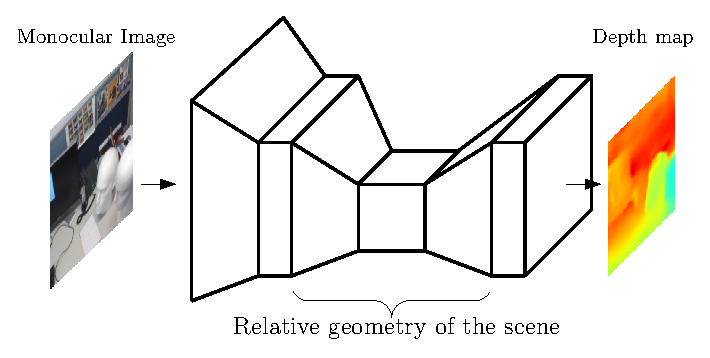
\includegraphics[width=0.5\linewidth]{images/intro/encoder_dec}
		\end{figure}	
		
		\vfill
		
		We learn the relative geometry of the scene to refine the query position and orientation.
\end{frame}

